\section{Αριθμητικές Μαγνητοϋδροδυναμικές εξομοιώσεις}
Η επίλυση ενός υδροδυναμικού προβλήματος με αριθμητικές μεθόδους είναι μια δύσκολή και πολύ απαιτητική διαδικασία. \todo{αναπτυξε το}

\subsection{Εξισώσεις Διατήρησης}
Οι εξισώσεις διατήρησης είναι χρονοεξαρτώμενα συστήματα μερικών διαφορικών εξισώσεων που έχουν τη γενική μορφή:
\begin{equation}
\label{eq:hyperbolicconservation}
\pdv{t} \bar{q}(x,t) + \pdv{x} \bar{f}(\bar{q}(x,t)) = 0 
\end{equation}
με $\bar{q}(x,t) \in \mathbb{R}^m$ ένα m-διάστατο άνυσμα των διατηρουμένων ποσοτήτων με  $\int_{-\infty}^{\infty} q_j (x,t) dx$ να είναι η ολική ποσότητα η οποία παραμένει σταθερή στο χρόνο t. 

Η $q_j(x,t)$ είναι ουσιαστικά η χωρική κατανομή (πυκνότητα) στο χρόνο $t$ η οποία γενικά μεταβάλλεται με το χρόνο.
Αυτή η μεταβολή περιγράφεται από τη συνάρτηση ροής $f_j(q(x,t))$. 
 
Το σύστημα \ref{eq:hyperbolicconservation} είναι η γενικότερη (μη γραμμική) μορφή των γραμμικών υπερβολικών εξισώσεων της μορφής:
\begin{equation}
\label{eq:linearhyperbolic}
\pdv{q}{t} +  \mathbf{A}\pdv{q}{x}  = 0 
\end{equation}
όπου $\mathbf{A}$ ένας τετραγωνικός διαγωνοποιήσιμος πίνακας με πραγματικές ιδιοτιμές.

Όπως και για τη μονοδιάστατη \todo{Λαθος} περίπτωση 
\begin{equation}
\label{eq:simple_advection}
\pdv{q}{t} +  u\pdv{q}{x}  = 0 
\end{equation}
η οποία έχει σαν λύση τη κυματική λύση D'Alembert
\begin{equation}
q(x,t)=q(x-ut,0)
\end{equation}
η γενική εξίσωση \ref{eq:linearhyperbolic} επιδέχεται αντίστοιχες κυματικές λύσεις.

Στη μη-γραμμική περίπτωση \ref{eq:hyperbolicconservation} το σύστημα λέγεται υπερβολικό αν ο ιακωβιανός πίνακας $\mathbf{J}(q)$ με στοιχεία $(i,j)$ τα $\pdv{f_i}{g_j}$ είναι αντίστοιχα διαγωνοποιήσιμος με πραγματικές ιδιοτιμές.

Τότε μπορούμε να γράψουμε το σύστημα των μη-γραμμικών εξίσωσεων στη μορφή:
\begin{equation}
\pdv{\bar{q}}{t} + \mathbf{J}(\bar{q}) \pdv{\bar{q}}{x} = 0 
\end{equation}

\subsection{Εξισώσεις Euler}
Οι εξισώσεις euler είναι ένα σύστημα μη-γραμμικών υπερβολικών μερικών διαφορικών εξισώσεων που περιγράφουν ένα ρευστό χωρίς ιξώδες και θερμική αγωγιμότητα\marginpar{Τα φαινόμενα διάχυσης (θερμική αγωγιμότητα, μοριακή διάχυση, ιξώδες) δίνουν όρους διάχυσης στη συνάρτηση ροής η οποία τώρα είναι της μορφής $f(q,q_x)$. Αποτέλεσμα αυτού είναι στο δεξί μέλος των εξισώσεων να εμφανίζονται όροι $\pdv*[2]{q}{x}$ και από υπερβολικές να γίνονται παραβολικές. Η πλήρης μορφή των υδροδυναμικών εξισώσεων δίνεται από τις εξισώσεις Navier-Stokes}.   
\begin{align}
&\pdv{\rho}{t} + \div(\rho \vec{u})=0 \label{eq:MassHD} && 
\texttt{Διατήρηση Μάζας} \\
&\pdv{t}(\rho  \vec{u})+\div(\rho  \vec{u}  \vec{u} +P)=0 && 
\texttt{Διατήρηση Ορμής} \label{eq:MomentumHD} \\
&\pdv{E}{t}+\div((E+P)\vec{u})=0 \label{eq:EnergyHD} && 
\texttt{Διατήρηση Ενέργειας}
\end{align}
με $E=\frac{P}{\gamma -1} +\frac{1}{2}\rho u^2$ η ενέργεια για ένα πολυτροπικό αέριο και $P$ η πίεση.

Σύμφωνα με τα προηγούμενα μπορούμε να γράψουμε το σύστημα στη μορφή \ref{eq:hyperbolicconservation}:
\begin{equation}
\pdv{t} \bar{q}(\vec{x},t) + \div\mathbf{f}(\bar{q}(\vec{x},t)) = 0 
\end{equation}
όπου 
\begin{equation}
\bar{q}(\vec{x},t)=\mqty(\rho \\ 
						\rho  \vec{u} \\
						E)
						=
						\mqty(q_1 \\ 
							  q_2 \\
							  q_3)
\end{equation}
και
\begin{equation}
\mathbf{f}(\bar{q}) = \mqty(\rho \vec{u} \\ 
						\rho \vec{u}\vec{u} + P \\
						\vec{u}(E+P))
					= \mqty(q_2 \\ 
						\frac{q_2 ^2}{q_1} +P(\bar{q}) \\
						\frac{q_2}{q_1} (q_3+P(\bar{q})))
\end{equation}
όπου $P(\bar{q})$ η καταστατική εξίσωση.


\subsection{Πηγές}
Μέχρι τώρα έχουμε υποθέσει ότι όλες οι διατηρούμενες ποσότητες, "διατηρούνται". Σε πραγματικές συνθήκες όμως υπάρχουν πηγές που προσθέτουν ή αφαιρούν (καταβόθρες) από τις ποσότητες μας. Μερικά παραδείγματα είναι:
\begin{itemize}
	\item Χημικές διεργασίες, ιονισμός και επανασύνδεση που ανταλλάσσουν / δημιουργούν / καταστρέφουν μάζες μεταξύ στοιχείων (διατήρηση της μάζας για πολλαπλά ρευστά)
	\item Εξωτερικές δυνάμεις όπως η βαρύτητα που λειτουργούν σαν πηγές στις εξισώσεις ορμής και ενέργειας.
	\item Μεταφορά θερμότητας μέσω ακτινοβολίας που λειτουργεί σαν πηγή (θέρμανση) ή καταβόθρα (ψύξη)
\end{itemize}
Οι εξισώσεις μας τότε αποκτούν τη μη ομογενή μορφή:
\begin{equation}
\pdv{t} \mathbf{q}(\vec{x},t) + \div\mathbf{f}(\mathbf{q}(\vec{x},t)) = S(\mathbf{q}(\vec{x},t))
\end{equation}

%\begin{marginfigure}
%	\label{fig:sodleveque}
%	\centering
%	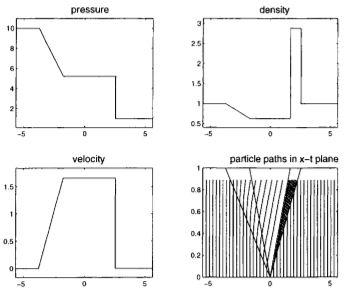
\includegraphics[width=1\linewidth]{Images/SODleveque}
%	\caption{Επίλυση του προβλήματος Riemann για τις μονοδιάστατες εξισώσεις Euler με αρχικές συνθήκες όπου η αρχική πίεση στα αριστερά είναι 10πλάσια της αρχικής πίεσης στα δεξιά ενώ οι αρχικές πυκνότητες μένουν ίδιες. Οι χαρακτηριστικές ταχύτητες είναι διαφορετικές (τελευταίο σχήμα) με αποτέλεσμα τα σωματίδια να πυκνώνουν και να δημιουργούν ένα κρουστικό κύμα πύκνωσης προς τα δεξιά, ενώ προς τα αριστερά δημιουργείται ένα κύμα αραίωσης. \cite{leveque_computational_1998}}
%\end{marginfigure}



\subsection{Αριθμητική επίλυση υπερβολικών εξισώσεων}
Η αριθμητική επίλυση των υπερβολικών εξίσωσεων αποτελεί μια δύσκολη διαδικασία
\subsubsection{Μέθοδος πεπερασμένων διαφορών}
Η βασική αρχή της μεθόδου των πεπερασμένων διαφορών -όπως και μεθόδων που πηγάζουν από αυτή και θα δούμε στη συνέχεια- είναι η διακριτοποιήση του χώρου και του χρόνου. Δηλαδή αναζητούμε μια προσεγγιστική τιμή των προς αναζήτηση ποσοτήτων σε συγκεκριμένα σημεία στο χώρο και στο χρόνο. Αν διακριτοποιήσουμε το χώρο κατα αποστάσεις $\Delta x=\Delta y = h$ και στο χρόνο $\Delta t=k$ τότε η προσεγγιστική τιμή στη θέση $(x_\mathrm{i},y_\mathrm{j})=(x_0+\mathrm{i}h,y_0+\mathrm{j}h)$ και στο χρόνο $t_\mathrm{n}=t_0+\mathrm{n}k$ θα είναι:
\begin{equation}
Q_{\mathrm{ij}}^\mathrm{n }\simeq q(x_\mathrm{i},y_\mathrm{j},t_\mathrm{n})
\end{equation}
Οπότε μια (για παράδειγμα μονοδιάτατη) μερική διαφορική εξίσωση της μορφής
\begin{equation}
\pdv{q}{t}+u\pdv{q}{x}=0
\end{equation} 
θα γράφεται:
\begin{equation}
\frac{Q_\mathrm{i}^\mathrm{n+1}-Q_\mathrm{i}^n }{k} + u \left( \frac{Q_\mathrm{i}^\mathrm{n+1}-Q_\mathrm{i}^\mathrm{n} }{k}  \right) =0
\end{equation}
άρα με βάση τις αρχικές συνθήκες $q_i^0$ μπορούμε να ολοκληρώσουμε στο χρόνο, άρα η λύση στο κελί με συντεταγμένες $\mathrm{ijn}$ θα είναι:
\begin{equation}
Q_{\mathrm{i}}^\mathrm{n+1} = Q_{\mathrm{i}}^\mathrm{n} -\frac{k}{h} u \left( Q_\mathrm{i}^\mathrm{n} - Q_\mathrm{i-1}^\mathrm{n} \right)
\end{equation} 

Αντίστοιχα στη περίπτωση ενός συστήματος εξισώσεων η λύση θα ήταν
\begin{equation}
Q_{\mathrm{i}}^\mathrm{n+1} = Q_{\mathrm{i}}^\mathrm{n} -\frac{k}{h} \mathbf{Α} \left( Q_\mathrm{i}^\mathrm{n} - Q_\mathrm{i-1}^\mathrm{n} \right)
\end{equation} 
με τον πίνακα $\mathbf{Α}$ να έχει θετικές ιδιοτιμές. 

Η τιμή των ποσοτήτων σε ένα κελί παρατηρούμε ότι εξαρτάται από τις τιμές των αμέσως γειτονικών κελιών. Η ακρίβεια μας τώρα είναι της τάξης του $h$ \todo{γιατί? Taylor}. Για να πετύχουμε μεγαλύτερη ακρίβεια μπορούμε να ανανεώνουμε τις ποσότητες $q_j$ με βάση πιο απομακρυσμένα κελιά, όπως για παράδειγμα η μέθοδος leapfrog:
\begin{equation}
Q_{\mathrm{i}}^\mathrm{n+1} = Q_{\mathrm{i}}^\mathrm{n-1} -\frac{k}{h} \mathbf{Α} \left( Q_\mathrm{i+1}^\mathrm{n} - Q_\mathrm{i-1}^\mathrm{n} \right)
\end{equation} 
ή να κρατήσουμε τους 3 πρώτους όρους από το αναπτύγμα Taylor $q(x,t+k)=q(x,t)+k\pdv{q}{t}(x,t)+\frac{1}{2}k^2 \pdv[2]{q}{t}$ τη μέθοδο Lax-Wendroff:
 
 \begin{equation}
 Q_{\mathrm{i}}^\mathrm{n+1} = Q_{\mathrm{i}}^\mathrm{n} -\frac{k}{2h} \mathbf{Α} \left( Q_\mathrm{i+1}^\mathrm{n} - Q_\mathrm{i-1}^\mathrm{n} \right) +\frac{k^2}{2h^2} \mathbf{Α}^2 \left( Q_\mathrm{i+1}^\mathrm{n} - 2Q_{\mathrm{i}}^\mathrm{n}+ Q_\mathrm{i-1}^\mathrm{n} \right)
 \end{equation} 
 
 Παρά το βαθμό ακρίβεια της κάθε μεθόδο μετάξυ των παρπαπάνω, οι μέθοδοι πεπερασμένων διαφορών δεν καταφέρνουν να διατηρήσουν τις ολοκληρώσιμες ποσότητες. Γι αυτό το σκοπό θα χρησιμοποιοήσουμε τις λεγόμενες μεθόδους πεπερασμένων όγκων.
 
\subsubsection{Μέθοδος Πεπερασμένων Όγκων}
Αντί για τη προσεγγιστική τιμή $Q_{\mathrm{i}}^\mathrm{n+1}$ της $q(x_\mathrm{i},t_\mathrm{n+1})$ σε ένα συγκεκριμένο σημείο θα ορίσουμε μια νέα αντίστοιχη τιμή για τη μέση τιμή της ποσότητας σε κάθε ένα διάστημα $C_\mathrm{i}=[x_\mathrm{i},x_\mathrm{i+1}]$ του χώρου μας με $x_\mathrm{i}=x_0+(i-1)h$. 

Άρα τώρα η τιμή $Q_{\mathrm{i}}^\mathrm{n}$ θα προσεγγίζει την μέση τιμή στο $\mathrm{i}$ διάστημα τη χρονική στιγμή $t_\mathrm{n}$
\begin{equation}
Q_{\mathrm{i}}^\mathrm{n} \simeq \frac{1}{h} \int _{C_\mathrm{i}} q(x,t_\mathrm{n})dx
\end{equation}






\subsection{Πρόβλημα Riemann}
Το πρόβλημα Riemann είναι η επίλυση ενός νόμου διατήρησης όπως τον έχουμε ορίσει παραπάνω με αρχικές συνθήκες όπου υπάρχει μια ασυνέχεια:
\begin{equation}
\bar{q}(x,0)=
\begin{cases}
\bar{q}_\mathrm{L} &\qq{για} x<0 \\
\bar{q}_R &\qq{για} x>0 
\end{cases}
\end{equation}

Όπως βλέπουμε χαρακτηριστικά και στο shock tube problem (\ref{fig:sodleveque}), λόγω της αρχικής ασυνέχειας και της μη-γραμμικότητας των εξισώσεων euler έχουμε σαν αποτέλεσμα τη δημιουργία κρουστικών κυμάτων.


\subsubsection{Γενική επίλυση του γραμμικού προβλήματος Riemann}
Η επίλυση του προβλήματος Riemann στη γραμμική περίπτωση (\ref{eq:linearhyperbolic}) βασίζεται στο μετασχηματισμό των ποσοτήτων $q$ στις λεγόμενες χαρακτηριστικές μεταβλητές $\bar{\xi}=\mathbf{R}^{-1}\bar{q}$ όπου $\mathbf{R}=(\bar{r}_1,\bar{r}_2,\cdots \bar{r}_m)$ ο πίνακας των ιδιοανυσμάτων του πίνακα $\mathbf{A}=\mathbf{R}\mathbf{\Lambda}\mathbf{R}^{-1}$. Με $\bar{\Lambda}=\mathtt{diag}(\lambda _1,\lambda _2,\cdots \lambda _m)$ ο διαγώνιος πίνακας των ιδιοτιμών.

Οι εξισώσεις τότε γράφονται:
\begin{equation}
\pdv{\bar{\xi}}{t} + \bar{\Lambda} \div\bar{\xi} =0
\end{equation} 
δηλαδή σαν ένα διαχωρισμένο σύστημα εξισώσεων της μορφής \ref{eq:simple_advection} με λύσεις:
\begin{equation}
\label{eq:xi_solution}
\xi_p  = \xi_p(x-\lambda _p t,0) 
\end{equation}
με $p=1...m$ για τις $m$ εξισώσεις (μονοδιάστατη περίπτωση). Οι $p$ χαρακτηριστικές καμπύλες δηλαδή καθορίζονται από τις ιδιοτιμές $\lambda _p$.

Άρα αν επιστρέψουμε στις αρχικές μεταβλητές:
\begin{equation}
\bar{q}(x,t) = \sum_{p=1}^{m} \xi_p(x-\lambda _p t,0)\bar{r}_p
\end{equation}

Για τις αρχικές συνθήκες του προβλήματος Riemann o μετασχηματισμός μας δίνει:
\begin{equation}
\xi_p (x,0) =
\begin{cases}
u^L_p &\qq{για} x<0 \\
u^R_p &\qq{για} x>0 
\end{cases}
\end{equation} 

άρα από \ref{eq:xi_solution}
\begin{equation}
\xi_p (x,t) =
\begin{cases}
u^L_p &\qq{για} x-\lambda _p t<0 \\
u^R_p &\qq{για} x-\lambda _p t>0 
\end{cases}
\end{equation} 

\begin{marginfigure}
	\label{fig:linearriemann-leveque}
	\centering
	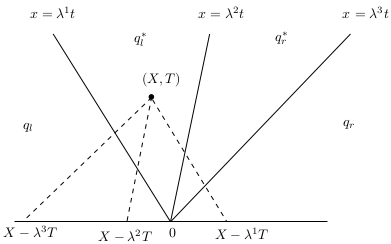
\includegraphics[width=1\linewidth]{Images/LinearRiemann-leveque}
	\caption{Λυση γραμμικου riemann}
\end{marginfigure}

φσαδα 

Άρα με αρχικές συνθήκες Riemann, βλέπουμε ότι η λύση για τις μετασχηματισμένη μεταβλητή $\xi _p$ σε ένα οποιαδήποτε σημείο εξαρτάται απόλυτα αό τη σχετική θέση σε σχέση με την αντίστοιχη χαρακτηριστική καμπύλη της $\lambda _p$.  

Καθώς διασχίζουμε τη καμπύλη αυτή ουσιαστικά μετακινούμαστε από τις συνθήκες $\xi^L_p$ στις $\xi^R_p$. Το άλμα αυτό υπακούει τις συνθήκες Rankine-Hugoniot \todo{Rankine-Hugoniot} άρα για κάθε σημείο μπορούμε τελικά να γράψουμε τη λύση.
\begin{equation}
\bar{q}(x,t)=q_L + \sum_{\lambda_p<x/t} (\xi ^R_P - \xi ^L_P) \bar{r_p}
			=q_R - \sum_{\lambda_p>x/t} (\xi ^R_P - \xi ^L_P) \bar{r_p}
\end{equation}
\todo{Επιλυση γραμμικου Riemann διαγραμμα}

\subsubsection{Επίλυση του μη γραμμικού προβλήματος Riemann}


\subsection{Κώδικας PLUTO}

